%% Font size %%
\documentclass[11pt]{article}

%% Load the custom package
\usepackage{Mathdoc}

%% Numéro de séquence %% Titre de la séquence %%
\renewcommand{\centerhead}{Chap. 7 : Parallélogrammes}

%% Spacing commands %%
\renewcommand{\baselinestretch}{1} \setlength{\parindent}{0pt}


\begin{document}

\section{Propriétés du parallélogramme}

\begin{definition}
Un parallélogramme est un quadrilatère ayant ses côtés opposés parallèles.
\end{definition}

\begin{exemple}
\begin{center}
\begin{tikzpicture}
\coordinate (A) at (0,0); \coordinate (B) at (3,0); \coordinate (D) at
(1,1.732); \coordinate (C) at ($(B)+(D)-(A)$);

\draw (A) -- (B) -- (C) -- (D) -- cycle;

\node[below left] at (A) {A}; \node[below right] at (B) {B};
\node[above right] at (C) {C}; \node[above left] at (D) {D};
\end{tikzpicture}
\end{center}
\end{exemple}

\begin{propriete}
Le point d'intersection des diagonales est le centre de symétrie du parallélogramme.
\end{propriete}

\begin{propriete}
Si un quadrilatère est un parallélogramme, alors
\begin{enumerate}
\item Ses diagonales se coupent en leur milieu ; 
\item ses côtés opposés sont de même mesure ; 
\item ses angles opposés sont de même mesure ; 
\item la somme des mesures de deux angles consécutifs est de 180\degre.
\end{enumerate}
\end{propriete}

\begin{exemple}
\begin{center}
\begin{tikzpicture}
\coordinate (A) at (0,0); \coordinate (B) at (3,0); \coordinate (D) at
(1,1.732); \coordinate (C) at ($(B)+(D)-(A)$);

\draw (A) -- (B) -- (C) -- (D) -- cycle;

\node[below left] at (A) {A}; \node[below right] at (B) {B};
\node[above right] at (C) {C}; \node[above left] at (D) {D};

\draw[dotted] (D) -- (B); \draw[dotted] (A) -- (C); 
\coordinate (I) at (intersection of A--C and D--B); 
\node[above] at (I) {I};
\end{tikzpicture}
\end{center}
\end{exemple}

\begin{remarque}
Dans le parallélogramme ci-dessus :
\begin{itemize}
\item Les diagonales $[DB]$ et $[AC]$ se coupent en leur milieux ;
\item les côtés $[DC]$, $[AB]$ et $[DA]$, $[CB]$ sont de même longueur
;
\item les angles $\widehat{DAB}$ et $\widehat{DCB}$ sont égaux, ainsi que $\widehat{ADC}$ et $\widehat{ABC}$ ;
\item la somme des angles consécutifs, par exemple $\widehat{DAB} + \widehat{ABC}$, est égale à $180^\circ$.
\end{itemize}
\end{remarque}

\section{Reconnaître un parallélogramme}

\begin{propriete}
Si un quadrilatère a ses diagonales qui se coupent en leur milieu, alors c'est un parallélogramme.
\end{propriete}

\begin{propriete}
Si un quadrilatère a des côtés opposés de même mesure, alors c'est un parallélogramme.
\end{propriete}

\begin{propriete}
Si un quadrilatère a deux côtés opposés de même mesure et parallèles, alors c'est un parallélogramme.
\end{propriete}

\begin{exemple}
\begin{center}
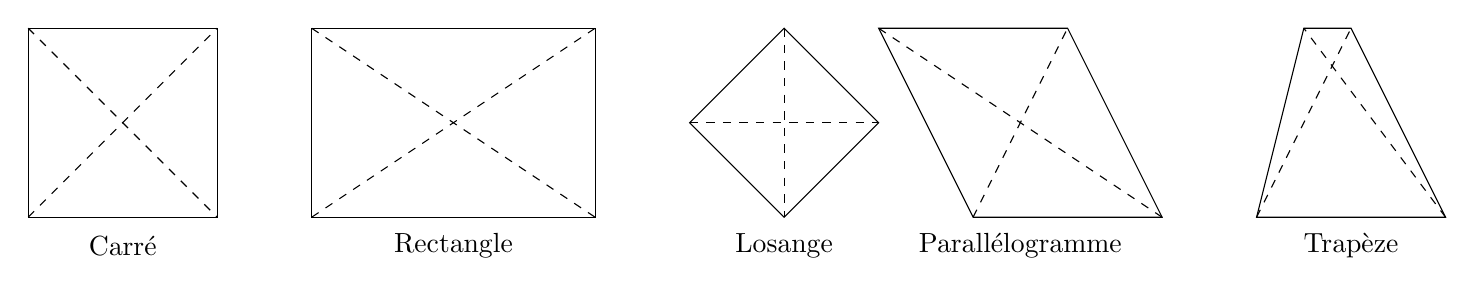
\begin{tikzpicture}[scale=1.2]

% Carré
\draw (0,0) rectangle (2,2); \draw[dashed] (0,0) -- (2,2); \draw[dashed] (0,2) -- (2,0); \node at (1, -0.3) {Carré};

% Rectangle
\draw (3,0) rectangle (6,2); \draw[dashed] (3,0) -- (6,2); \draw[dashed] (3,2) -- (6,0); \node at (4.5, -0.3) {Rectangle};

% Losange
\draw (7,1) -- (8,2) -- (9,1) -- (8,0) -- cycle; \draw[dashed] (7,1) -- (9,1); \draw[dashed] (8,2) -- (8,0); \node at (8, -0.3) {Losange};

% Parallélogramme
\draw (10,0) -- (12,0) -- (11,2) -- (9,2) -- cycle; \draw[dashed] (10,0) -- (11,2); \draw[dashed] (12,0) -- (9,2); \node at (10.5, -0.3) {Parallélogramme};

% Trapèze
\draw (13,0) -- (15,0) -- (14,2) -- (13.5,2) -- cycle; \draw[dashed] (13,0) -- (14,2); \draw[dashed] (15,0) -- (13.5,2); \node at (14, -0.3) {Trapèze};

\end{tikzpicture}
\end{center}
\end{exemple}

\section{Méthode de construction}

\begin{exemple}
Pour construire un parallélogramme $ABCD$ :
\begin{enumerate}
\item Tracer un segment $[AB]$ de longueur donnée.
\item Tracer un angle $\widehat{BAC}$ de mesure donnée.
\item Tracer un segment $[AD]$ de longueur donnée.
\item Compléter le quadrilatère en traçant $[DC]$ parallèle à $[AB]$ et $[BC]$ parallèle à $[AD]$.
\end{enumerate}
\end{exemple}

\begin{center}
\begin{tikzpicture}
\coordinate (A) at (0,0); \coordinate (B) at (3,0); \coordinate (D) at
(1,1.732); \coordinate (C) at ($(B)+(D)-(A)$);

\draw (A) -- (B) -- (C) -- (D) -- cycle;

\node[below left] at (A) {A}; \node[below right] at (B) {B};
\node[above right] at (C) {C}; \node[above left] at (D) {D};
\end{tikzpicture}
\end{center}

\section{Quadrilatères particuliers}

\begin{definition}
Rappels de sixième :
\begin{enumerate}
\item Un rectangle est un quadrilatère qui a quatre angles droits ;
\item Un losange est un quadrilatère qui a quatre côtés de même
longueur ;
\item Un carré est un quadrilatère qui a quatre angles droits et
quatre côtés de même longueur.
\end{enumerate}
\end{definition}

\begin{propriete}
\begin{enumerate}
\item Si un quadrilatère est un rectangle, alors ses diagonales sont
de même longueur ; 
\item Si un quadrilatère est un losange, alors ses diagonales sont
perpendiculaires ; 
\item Si un quadrilatère est un carré, alors ses diagonales sont perpendiculaires et de même longueur.
\end{enumerate}
\end{propriete}

\begin{remarque}
Le rectangle, le losange et le carré sont des parallélogrammes particuliers. En effet, ils ont tous leurs côtés opposés parallèles.
\end{remarque}



\end{document}

% Local Variables:
% gptel-model: deepseek-chat
% gptel--backend-name: "DeepSeek"
% gptel--bounds: ((491 . 812) (1326 . 1779) (2034 . 2054) (2062 . 2092) (2100 . 2111) (2119 . 2180) (2188 . 2196) (2204 . 2265) (2733 . 3533) (3596 . 4310))
% End:
